\section{Программное обеспечение IoT}
Программное обеспечение IoT обращается к своим ключевым областям работы в сети и действиям с помощью платформ, встроенных
системы, партнерские системы и промежуточное ПО. Эти индивидуальные и основные приложения
отвечает за сбор данных, интеграцию устройств, аналитику в реальном времени, приложения и
расширение процесса в сети IoT. Они используют интеграцию с критически важными бизнес-системами
(например, системы заказов, робототехника, планирование и т. д.) при выполнении связанных задач.

\subsection{Сбор информации}
Это программное обеспечение управляет датчиками, измерениями, фильтрацией световых данных, безопасностью световых данных и
агрегация данных. Он использует определенные протоколы, чтобы помочь датчикам подключаться к данным в реальном времени.
межмашинные сети. 
\begin{figure}[h!]
    \centering
    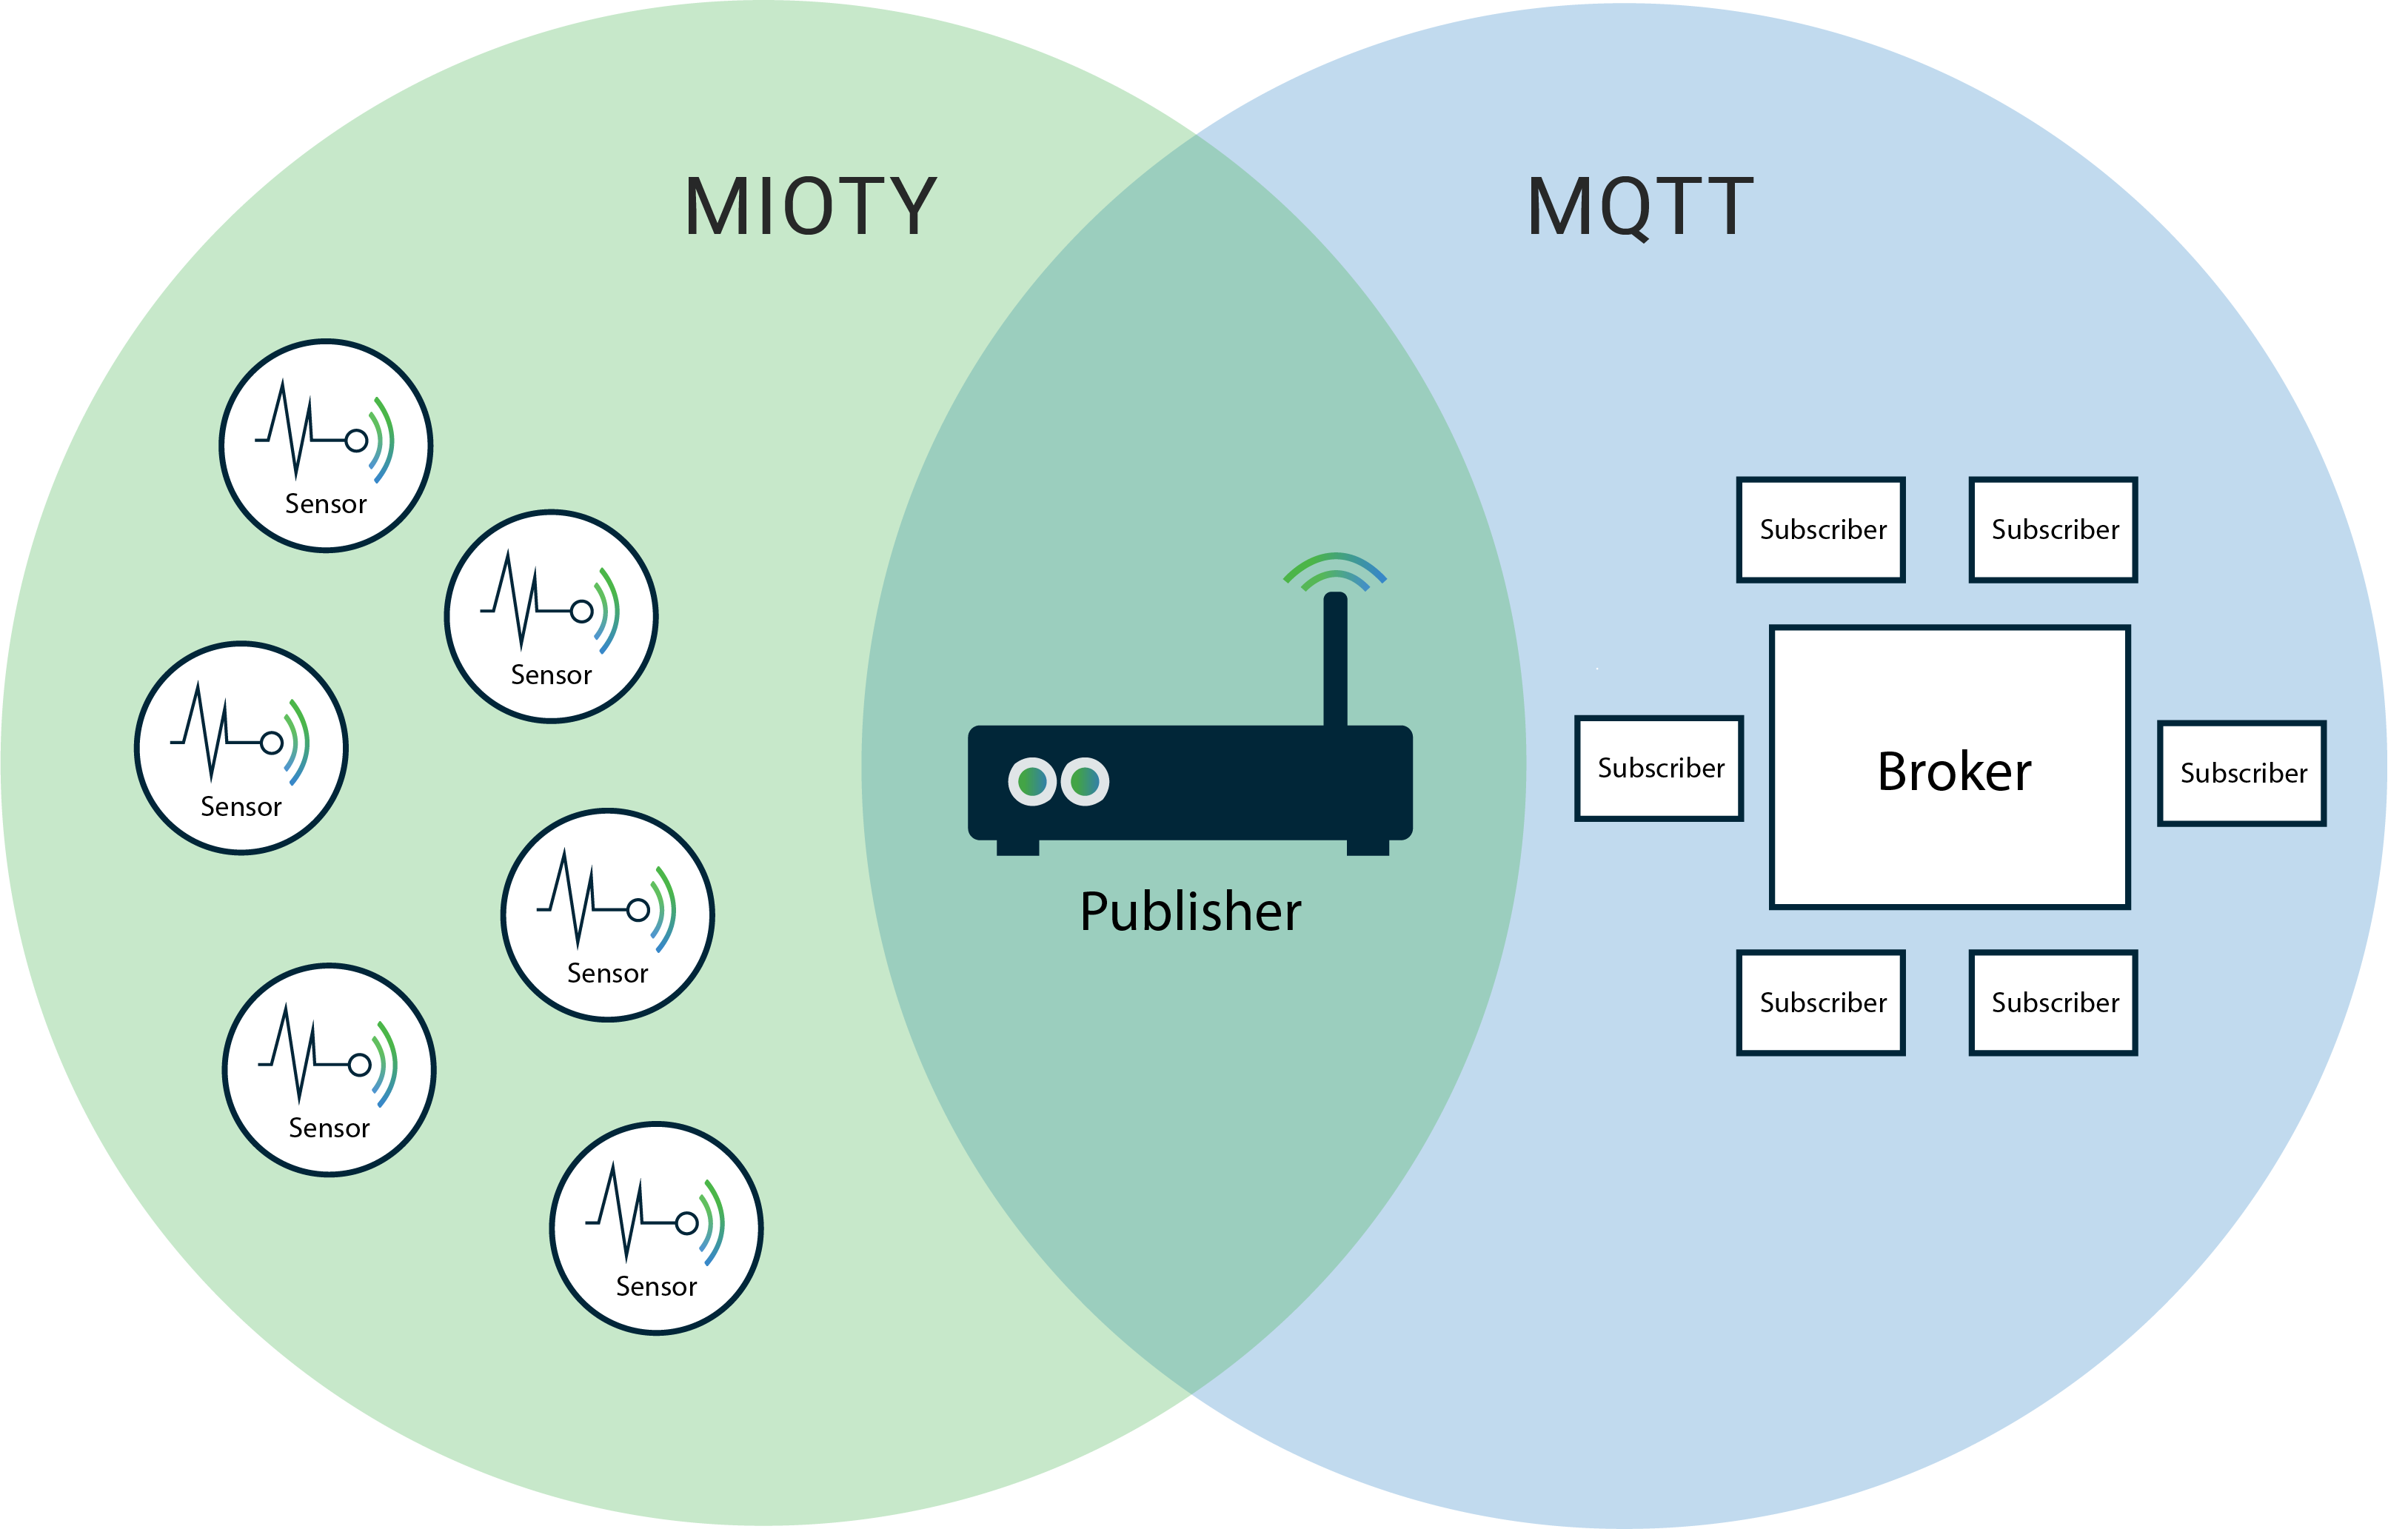
\includegraphics[scale=0.3]{data_collecting.png}
    \caption{Диаграмма сбора данных в системе IoT}
    \label{fig:section5:data_collecting}
\end{figure}
Затем он собирает данные с нескольких устройств и распределяет их в
соответствии с настройками. Он также работает в обратном порядке, распределяя данные по устройствам. Система
в конечном итоге передает все собранные данные на центральный сервер.

\subsection{Интеграция устройств}
Программное обеспечение, поддерживающее интеграцию, связывает (зависимые отношения) все системные устройства для создания
тело системы IoT. Это обеспечивает необходимое сотрудничество и стабильную сеть между
устройства. Эти приложения являются определяющей программной технологией сети IoT, поскольку
без них это не система IoT. Они управляют различными приложениями, протоколами и
ограничения каждого устройства для обеспечения связи.\cite{IoTAzure}

\subsection{Аналитика в реальном времени}
Эти приложения берут данные или входные данные с различных устройств и преобразуют их в жизнеспособные действия или действия.
четкие закономерности для человеческого анализа. 
\begin{figure}[h!]
    \centering
    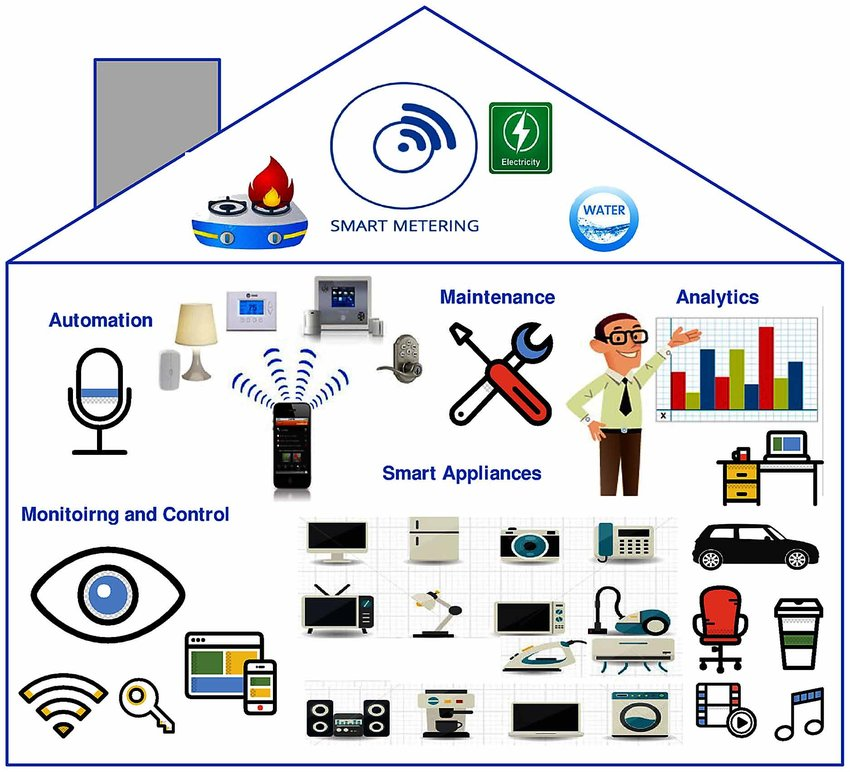
\includegraphics[scale=0.3]{realtime.png}
    \caption{Обработка данных и дальнейшая взаимосвязь между устройствами}
    \label{fig:section5:realtime}
\end{figure}
Они анализируют информацию на основе различных настроек и
проекты для выполнения задач, связанных с автоматизацией, или предоставления данных, требуемых промышленностью.

\subsection{Применение и расширение процесса}
Эти приложения расширяют возможности существующих систем и программного обеспечения, позволяя
эффективная система. Они интегрируют предопределенные устройства для определенных целей, таких как разрешение определенных
доступ к мобильным устройствам или инженерным приборам. Он поддерживает повышенную производительность и многое другое
точный сбор данных.